\documentclass{beamer}

%% Language and font encodings
\usepackage[english]{babel}
\usepackage[utf8x]{inputenc}
\usepackage[T1]{fontenc}


%% Useful packages
\usepackage{amsmath,amssymb}
\usepackage{mathtools}
\usepackage{graphicx}
\usepackage{amsthm} % for proof pkg
\usepackage{proof}
\usepackage[colorinlistoftodos]{todonotes}
\usepackage{tikz}
\usepackage{graphicx}
\usepackage{caption}
\usepackage{subcaption}
\newcommand*\circled[1]{\tikz[baseline=(char.base)]{
             \node[shape=circle,draw,inner sep=0.2pt] (char) {#1};}}
\usetheme{Boadilla}

\newtheorem{pf_idea}{Proof Idea}
\newtheorem{idea}{ }

\newcommand{\RR}{\mathbb{R}}


\title{ADP using Fluid and Diffusion Approximations}
\author{Ariah Klages-Mundt}
\date{December 4, 2017}

\begin{document}

\begin{frame}
ORIE 6590 Project
\titlepage

\begin{center}
Chen et. al.,
	\emph{Approximate Dynamic Programming using Fluid and Diffusion Approximations with Applications to Power Management},
	Proceedings of the 48h IEEE Conference on Decision and Control held jointly with 28th Chinese Control Conference (2009)
\end{center}
\end{frame}

%%%%%%%%%%%%%%%%%%%%%%%%%%%%%%%%%%%%%%%%%%
\frame{
\textbf{Question:} How to determine a good feature space for approximate DP algorithms?

\vspace{0.5cm}
\textbf{This paper:} Use approximations from simplified versions of the problem to choose basis

\vspace{0.5cm}
Outline of this talk:
\begin{enumerate}
\item Speed scaling problem
\item Fluid approximation
\item Diffusion approximation
\item LSTD using fluid and diffusion basis
\end{enumerate}
}


%%%%%%%%%%%%%%%%%%%%%%%%%%%%%%%%%%%%%%%%%%
\frame{
\frametitle{Idea behind fluid and diffusion models}

\begin{idea}
\textbf{Fluid model:}
Scale time, state by $n$: analogous to SLLN
$$\frac{1}{n} X(nt) \rightarrow \bar X(t)$$
\end{idea}

\begin{idea}
\textbf{Diffusion model:}
Scale time by $n$, state by $\sqrt{n}$: analogous to CLT
$$\sqrt{n} \left( \frac{1}{n} X(nt) - \bar X(t) \right) = \frac{X(nt) - \bar X(nt)}{\sqrt{n}} \rightarrow \hat X(t)$$
\end{idea}

\vspace{0.5cm}
Then think of $\bar X(t) + \hat X(t)$ as an approximation to $X(t)$
}

%%%%%%%%%%%%%%%%%%%%%%%%%%%%%%%%%%%%%%%%%%
\frame{
\frametitle{Speed scaling problem}

\begin{idea}
\textbf{Problem:} Control computer processing speed to balance energy and job delay costs. Single server queue with controllable service rate.
\end{idea}

For $t=0,1,2,\ldots$,
\begin{itemize}
\item $A(t)$ = i.i.d. job arrivals
\item $X(t)$ = queue length (system state)
\item $U(t)$ = service rate (the action to take).
\end{itemize}

\vspace{0.5cm}
States evolve as $X(t+1) = X(t) - U(t) + A(t+1)$

\vspace{0.5cm}
Cost function $c(x,u) = x + \beta \mathcal{P}(u)$ with $\beta>0$.

For most part, use $c(x,u) = x + \frac{1}{2} u^2$
}


%%%%%%%%%%%%%%%%%%%%%%%%%%%%%%%%%%%%%%%%%%
\frame{
\frametitle{Average cost problem}

For $h:\mathbb{R} \rightarrow \mathbb{R}$, \textbf{differential generator} $\mathcal{D}_u$ is
$$\begin{aligned}
\mathcal{D}_u h(x) &:=  \mathbf{E}\Big[ h\Big(X(t+1)\Big) - h\Big(X(t)\Big) \hspace{0.1cm} \vert \hspace{0.1cm} X(t) = x, U(t) = u \Big] \\
	&= \sum_j P_{xj}(u) h(j) - h(x)
\end{aligned}$$

\begin{idea}
\textbf{Average Cost Optimality Eq.} (ACOE)
$$\min_u \Big( c(x,u) + \mathcal{D}_u h^*(x) \Big) = \eta^*$$

Countable state space constraint: $\forall u, x$, $\lim_{n \rightarrow \infty} \frac{1}{n} \mathbf{E}_x^u | h^*(x_n)| = 0$
\end{idea}
}




%%%%%%%%%%%%%%%%%%%%%%%%%%%%%%%%%%%%%%%%%%
\frame{
\frametitle{Fluid model}

\begin{idea}
$$\begin{aligned}
\frac{d}{dt} x(t) &= \bar f(x(t),u(t)) = \mathbf{E}[f(x,u,w(1))], \hspace{2cm} x(0) \in X \\
	&= -u(t) + \alpha
\end{aligned}$$
\end{idea}

\vspace{0.5cm}
$$\mathcal{D}_u^F h(x) = \frac{d}{dt} h(x(t)) \vert_{t=0} = \nabla h(x) \cdot \bar f(x,u) \hspace{0.5cm} u(0)=u, x(0)=x$$


\begin{idea}
\textbf{Motivation:} Taylor series expansion. if $J^*$ is smooth, then
$$\begin{aligned}
\mathcal{D}_u J^* &\approx \mathbf{E} \Big[ \nabla J^*(X(0))(X(1)-X(0)) \vert X(0)=x, U(0)=u \Big] \\
	&= \nabla J^*(x) \bar f(x,u) \\
	&= \mathcal{D}_u^F J^*
\end{aligned}$$
\end{idea}
}




%%%%%%%%%%%%%%%%%%%%%%%%%%%%%%%%%%%%%%%%%%
\frame{
\frametitle{Fluid model}

\begin{idea}
\textbf{Total Cost Optimality Eq.} (TCOE)
$$\min_u \Big(c(x,u) + \mathcal{D}_u^F J^*(x)\Big) = 0$$
Supposing $J^*$ finite, solved with
$$J^*(x) = \inf_u \int_0^\infty c(x(t),u(t)) dt, \hspace{2cm} x(0)=x \in X$$
\end{idea}

\vspace{0.5cm}
We want $J^*$ to approximate the ACOE solution in a meaningful way
}



%%%%%%%%%%%%%%%%%%%%%%%%%%%%%%%%%%%%%%%%%%
\frame{
\frametitle{Fluid approximation}
Consider cost functions $c(x,u) = x + \beta([u-\alpha]_+)^\varrho,$ where
\begin{itemize}
\item $[\cdot]_+ = max(0,\cdot)$, $\beta>0$,
\item $\varrho>0$ integer
\item $c(0,\alpha)=0$
\end{itemize}

\begin{theorem}
$J^*$ approximately solves ACOE. In particular, there is a modified cost function $c^0 \approx c$ (with bounded error) and corresponding $\eta^0$ such that $J^*$ satisfies ACOE
$$\min_u \Big( c^0(x,u) + P_u J^*(x) \Big) = J^*(x) + \eta^0$$ 
\end{theorem}
}



%%%%%%%%%%%%%%%%%%%%%%%%%%%%%%%%%%%%%%%%%%
\frame{
\frametitle{Fluid approximation}

\begin{pf_idea}
Pick $\eta^0>0$ arbitrary and define error functions
$$\begin{aligned}
\varepsilon(x,u) &= c(x,u) - J^*(x) + P_u J^*(x), \\
\underline \varepsilon(x) &= \min_u \varepsilon(x,u)
\end{aligned}$$

$c^0(x,u) := c(x,u) - \underline \varepsilon(x) + \eta^0$, then $J^*$ satisfies ACOE (easy check)

\textbf{Lower bound} on $c^0-c$: use convexity of $J^*$

\textbf{Upper bound} on $c^0-c$:
\begin{itemize}
\item From MVT, for some $\bar X$ with value between $x$ and $x-u+A(1)$,
$$\begin{aligned}
\mathcal{D}_u J^*(x) &:= \mathbf{E} \Big[ J^*(X(1)) - J^*(X(0)) \vert X(0)=x, U(0)=u\Big] \\
	&= \nabla J^*(x) \cdot (-u + \alpha) + \frac{1}{2} \mathbf{E}\Big[ \nabla^2 J^*(\bar X) \cdot (-u + A(1))^2\Big].
\end{aligned}$$
\item Use error from fluid optimal policy and non-increasing $\nabla^2 J^*$
\end{itemize}
\end{pf_idea}
}





%%%%%%%%%%%%%%%%%%%%%%%%%%%%%%%%%%%%%%%%%%
\frame{
\frametitle{Diffusion model}

\begin{idea}
$dX(t) = \bar f\Big( X(t), U(t)\Big)dt + \sigma\Big( U(t)\Big) dN(t) + dI(t),$ \\ where
$N$ is BM, $I$ is reflection process
\end{idea}

$\mathcal{D}_u$ defined over $C^2$ fns. $g:\RR_+ \rightarrow \RR_+$ \\
restricted to $\nabla g(x) \vert_{x=0} = 0$ $\implies$ $I$ term vanishes in Ito's Lemma
$$\mathcal{D}_u g(x) = \nabla g(x) \cdot \bar f(x,u) + \frac{1}{2} \sigma^2(u) \nabla^2 g(x)$$

\begin{idea}
\textbf{Motivation:} 2nd order Taylor series approximation (previous slide), which also suggests
$$\sigma^2(u) = \mathbf{E}\Big[ (u-A(1))^2\Big] = u^2 - 2\alpha u + m_A^2$$
\end{idea}
}



%%%%%%%%%%%%%%%%%%%%%%%%%%%%%%%%%%%%%%%%%%
\frame{
\frametitle{Diffusion approximation}
Under $c(x,u) = x + \frac{1}{2}u^2$, optimal policy is $u^*(x) := \frac{\nabla h^*(x) + \alpha \nabla^2 h^*(x)}{1+\nabla^2 h^*(x)}$ \\
$u^* \geq 0$ (valid policy) by $h^*$ convexity and boundary condition

\vspace{1cm}
Fluid TCOE has solution $J^*(x) = \alpha x + \frac{1}{3} \left( (2x + \alpha^2)^{3/2} - \alpha^3 \right)$


\begin{theorem}
$h^0(x) = J^*(x) + \frac{1}{2}x$ approximately solves the diffusion ACOE. In particular, there is a modified cost function $c^0 \approx c$ (with bounded error) such that $h^0$ solves the ACOE exactly.
\end{theorem}

}



%%%%%%%%%%%%%%%%%%%%%%%%%%%%%%%%%%%%%%%%%%
\frame{
\frametitle{Diffusion approximation}

\begin{pf_idea}
Let $c^0(x,u) = c(x,u) + \frac{1}{8} \left( \frac{y}{y+1} - 4 \frac{\sigma_A^2}{y}\right) + \eta^0$, where
$\sigma_A^2$ variance of $A$, $y:= (2x+\alpha^2)^{1/2}$, $\eta^0>0$ arbitrary constant

\vspace{0.5cm}
Optimal average cost of $c^0$ is $\eta^0$ (fixed point equation)

\vspace{0.3cm}
$|c^0(x,u) - c(x,u)|$ is uniformly bounded over $x,u$

\vspace{0.3cm}
\textbf{Issue:} $h^0$ doesn't satisfy boundary condition $\nabla h^0(x) \vert_{x=0} = 0$

\textbf{Resolution:} decaying exponential perturbation for some $\nu>0$
$$h^{00}(x) = h^0(x) - \left(2\alpha + \frac{1}{2}\right) \nu e^{-x/\nu},$$
$h^{00}$ solves diffusion ACOE with some $c^{00}$ that retains the uniform boundedness of $c^{00}(x,u) - c(x,u)$
\end{pf_idea}
}




%%%%%%%%%%%%%%%%%%%%%%%%%%%%%%%%%%%%%%%%%%
\frame{
\frametitle{LSTD}

\begin{idea}
In summary:
\begin{itemize}
\item $J^*$ approximates $h^*$ (+caveats)
\item $h^0(x) = J^*(x) + \frac{1}{2}x$ approximates $h^*$ for diffusion
\end{itemize}
\end{idea}

\vspace{1cm}
Together, this suggests a basis for $h^*$:
$$\phi^1(x) = J^*(x), \hspace{1cm} \phi^2(x) = x$$
}


%%%%%%%%%%%%%%%%%%%%%%%%%%%%%%%%%%%%%%%%%%
\frame{
\frametitle{Computational setup}

$A(t) = \Delta_A G(t)$ for $t\geq 1$ where
\begin{itemize}
\item $G$ geometrically distributed with $p_A = 0.96$
\item $\Delta_A = \frac{1}{24}$
\end{itemize}

\vspace{0.5cm}
$X = \{ \Delta_A m \vert m = 0,\ldots,480\}$

\vspace{0.5cm}
$X(t+1) = \Big[ X(t) - U(t) + A(t+1)\Big]$ projected onto interval $[0,20]$.

\vspace{0.5cm}
$U(t)$ restricted to non-negative integer multiples of $\Delta_A$

\vspace{0.5cm}
$c(x,u) = x + \frac{1}{2}u^2$
}



%%%%%%%%%%%%%%%%%%%%%%%%%%%%%%%%%%%%%%%%%%
\frame{
\frametitle{Computational results: value iteration}

\begin{center}
\begin{figure}
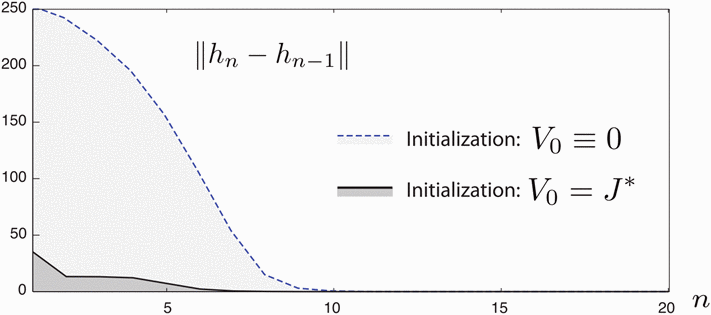
\includegraphics[width=10cm]{value_iter_converge}
\caption{Convergence of Value Iteration. $J^*$ is good initial guess.}
\end{figure}
\end{center}
}



%%%%%%%%%%%%%%%%%%%%%%%%%%%%%%%%%%%%%%%%%%
\frame{
\frametitle{Computational results: fluid approximation}

\begin{center}
\begin{figure}
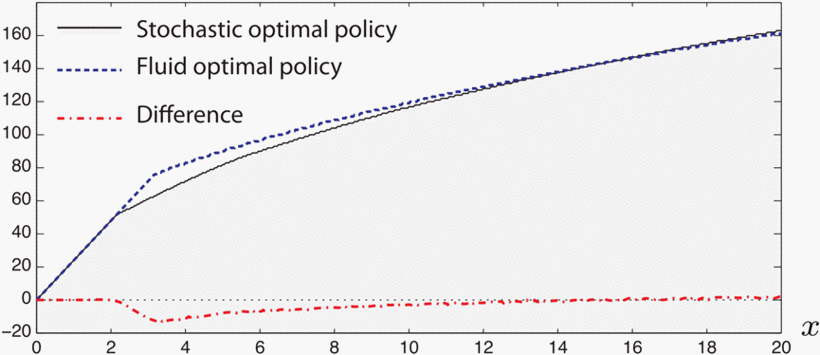
\includegraphics[width=10cm]{fluid_optimal_compare}
\caption{Optimal policy vs. fluid optimal policy}
\end{figure}
\end{center}
}



%%%%%%%%%%%%%%%%%%%%%%%%%%%%%%%%%%%%%%%%%%
\frame{
\frametitle{Computational results: LSTD approximation}

\begin{center}
\begin{figure}
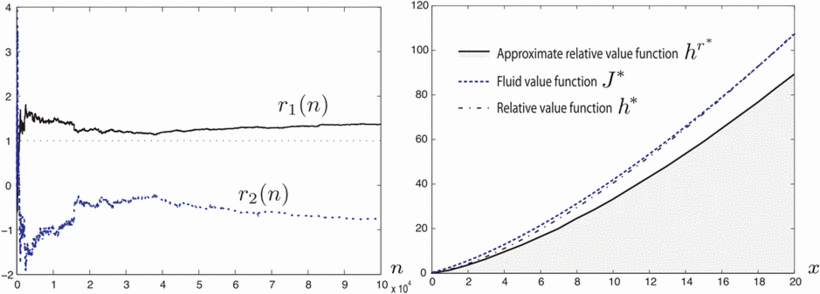
\includegraphics[width=10cm]{lstd_quad}
\caption{Simulation results. Left shows coefficients for basis functions. Right shows final approximations of $h^*$.}
\end{figure}
\end{center}

100,000 iterations of LSTD \\
Initial condition $r(0) = (0,0)^T$
}



%%%%%%%%%%%%%%%%%%%%%%%%%%%%%%%%%%%%%%%%%%
\frame{
\frametitle{Computational results: LSTD approximation}

Now use different cost function:
$\varrho = 15$, $\beta = 1/\varrho$.



\begin{center}
\begin{figure}
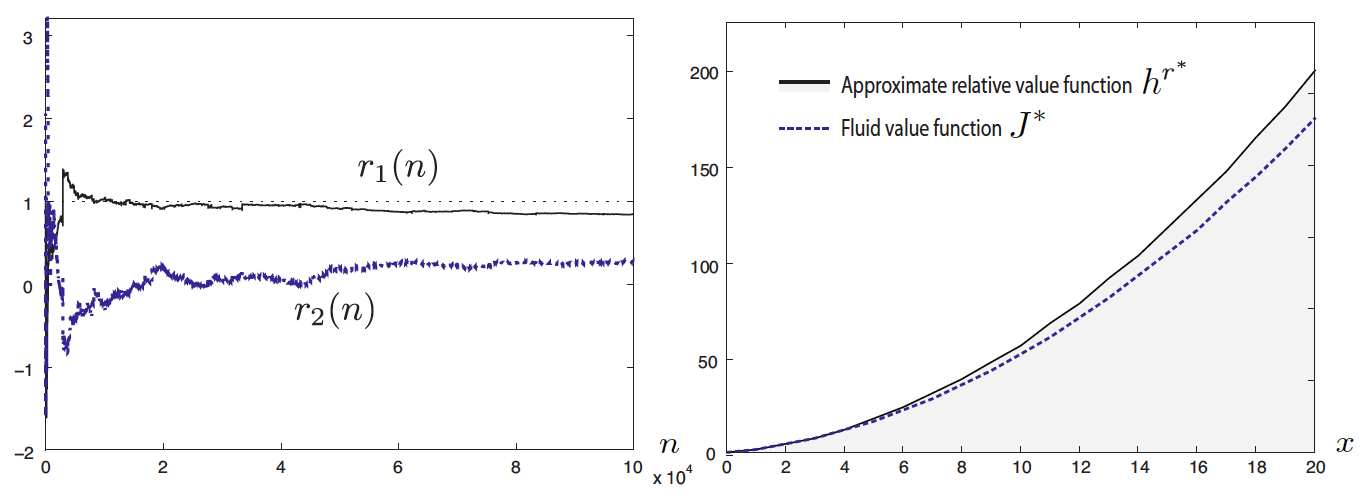
\includegraphics[width=10cm]{lstd_15}
\caption{Simulation results using $\varrho=15$ cost function. Left shows coefficients for basis functions. Right shows final approximations of $h^*$.}
\end{figure}
\end{center}
}


%%%%%%%%%%%%%%%%%%%%%%%%%%%%%%%%%%%%%%%%%%
\frame{
\frametitle{Computational results: PIA convergence}

\begin{center}
\begin{figure}
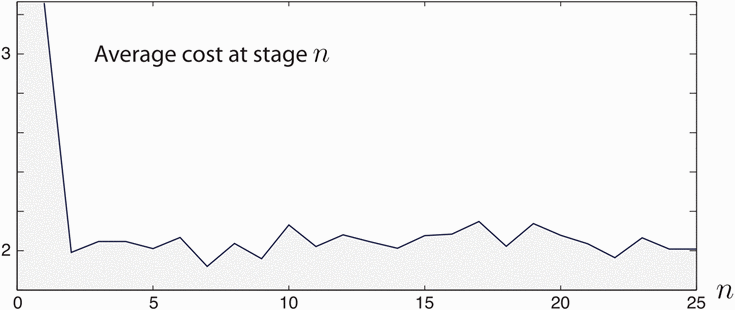
\includegraphics[width=10cm]{lstd_converge}
\caption{Estimated average cost from LSTD policy iteration with quadratic cost function. Fits idea that LSTD tends to converge quickly if we have a good basis.}
\end{figure}
\end{center}

Initial policy $u^0(x) = \min (x,1)$ for $x\geq 0$ for policy iteration with LSTD
}


%%%%%%%%%%%%%%%%%%%%%%%%%%%%%%%%%%%%%%%%%%
\frame{
\frametitle{Discussion}

\textbf{What's good:}
\begin{itemize}
\item Fluid-Diffusion basis works well in computations
\item Some theoretical justification for why fluid-diffusion approximations are reasonable
\item Extend some theoretical results to other cost functions (e.g., more general polynomials and exponentials)
\end{itemize}

\vspace{0.5cm}
\textbf{What's questionable/unaddressed:}
\begin{itemize}
\item Caveats on cost function in fluid model theoretical results
\item Are the basis functions counterintuitive, not something would have tried anyway?
\item Does method like this generalize well to other problems?
\item The computational problem considered isn't that difficult to solve. Is there a difficult problem that this method helps us to solve?
\end{itemize}


}










\end{document}